% %!TEX root = ../report.tex

\newcommand{\bo}[1]{\textbf{#1}}

\chapter{Architecture evaluation}

\label{ch:evaluation}
In this chapter the software architecture will be evaluated. This document started with a requirement analysis. The requirements which are defined in chapter 3 are checked if they are fulfilled in the software architecture. Another part in this chapter is the architecture evaluation using Architecture Tradeoff Analysis Method (ATAM). The architectural risks can be exposed that can harm the organization's business goals.

\section{Requirements validation}

A summary of the verification of the requirements from chapter 3 is given in this section. A table in which all the requirements get verified individually, can be found in appendix \ref{append:reqeval}.\\
The requirements validation shows that the functional requirements are met with this architecture. For the non-functional requirements there are a few requirements that have the status unknown, meaning there were complications in the verification.

%The requirements from chapter 3 are evaluated in this section. The section is split according to chapter 3. First the functional requirements, following the commercial requirements, and at the end the technical non-functional requirements.



%%!TEX root = ../report.tex

%############################################################
%## FUNCTIONAL 
%############################################################

\subsection{Functional requirements evaluation}

\begin{longtable}{llllL{\tw{0.1}}L{\tw{0.4}}}
    \bo{Nr.} & \bo{Priority} & \bo{Fulfilled} & \bo{Decision} & \bo{Chapter} & \bo{Remarks} \\ \toprule \endhead

    %		INTR-1 & Must     & Yes      &~\ref{subsec:external-system} & Fulfilled by using several weather forecast API providers.       \\ \midrule \midrule
    %The system is able to receive input from water level sensors.
    ~\ref{fr:receive-waterlevel} 
    & Must     
    & Yes
    & ~\ref{hw:1}, ~\ref{hw:2}, ~\ref{hw:3} 
    & ~\ref{sec:hardware-overview},~\ref{subsubsec:components}
    ,~\ref{subsec:logicalview} 
    & Fulfilled by the system providing a REST server the arduino sensor systems can use to post the sensor data to. \\ \midrule

    %The system is able to receive input from the dike sensors.
    ~\ref{fr:receive-pressure}
    & Must
    & Yes
    & ~\ref{hw:2}
    &~\ref{sec:hardware-decisions} ~\ref{hw:2}
    & Fulfilled by having arduino systems sent the dike sensor values over a cabled network to the central system's REST server \\ \midrule

    %The system is able to perform an analysis for the parameters of the dike sensors based on the input from the dike sensors.
    %TODO This has to be explained better i guess.
    ~\ref{fr:analyze-pressure}  
    & Must     
    & Yes        
    & ~\ref{hw:1}
    & ~\ref{subsec:logicalview}, ~\ref{subsec:view-process} 
    & Fulfilled, algorithm uses paramaters of dike sensors. \\ \midrule

    %FR-5 Must The system can store the sensor data.
    ~\ref{fr:store-sensordata}  
    & Must     
    & Yes        
    & ~\ref{dec:6}
    & ~\ref{sec:hardware-overview}, ~\ref{subsec:implementview}, ~\ref{subsec:databaseview}
    & Fulfilled by using an ElasticSearch database that is capable of storing all the data needed.\\ \midrule 

    ~\ref{fr:retrieve-sensordata}
    & Must
    & Yes
    & ~\ref{dec:6}
    & ~\ref{subsec:implementview}, ~\ref{subsec:databaseview}
    &Fulfilled by using an Elasticsearch database that is very robust, high available and scalable. Thereby enhancing the ability to store and receive data at all times. \\ \midrule

    %		%The system retrieves weather forecasting data from weather forecasting services,
    %which consists of predictions about the precipitation, wind data and tide information.
    %This is used by the system to help in determining when a flood becomes imminent
    ~\ref{fr:receive-weather}
    & Must
    & Yes
    & 
    &~\ref{subsec:external-system}
    & Fulfilled by the system contacting several API's to base the decisions on. \\ \midrule 

    %The system is able to detect when a flood is imminent by combining the retrieved
    %sensor data and weather forecasting data.
    ~\ref{fr:detect-flood}
    & Must
    & Yes
    &
    &~\ref{subsec:logicalview}, ~\ref{subsubsec:proc-floodmonitor}
    & Fulfilled by the system using Longitudinal Data Analysis to correlate the sensor data with the forecast data \\ \midrule 

    %		%The system retrieves geographic information, consisting of road data, terrain height
    %data and demographic data (number of civilians living in affected area) from an
    %external API.
    ~\ref{fr:receive-geographic}
    & Must
    & Yes
    &
    &~\ref{subsec:external-system}
    & Fulfilled by the system contacting an external GEO API over TCP/IP\\ \midrule

    %		%The system computes the area affected by a flood, in zones of 5 by 5 km, by using the
    %location data of the sensors and geographic information.
    ~\ref{fr:compute-area}
    & Must
    & Yes
    & ~\ref{dec:6}
    & ~\ref{subsec:database-data},~\ref{subsec:external-system}
    & Fulfilled by the system storing the geographical data in an ElasticSearch database, capable of performing queries to get the specified area \\ \midrule 

    %		%The system is able to perform an analysis, resulting in an estimated expected water
    %level for areas which are affected by a flood, based on the water level sensor data,
    %geographic data and weather forecast information.
    ~\ref{fr:analyze-waterlevel}
    & Must
    & Yes
    &
    &~\ref{sec:elaboratedmodel} ~\ref{subsec:logicalview}
    & Fulfilled by using several different external API's for additional information together with a correlation algorithm and other analysis algorithms \\ \midrule 

    %The system estimates how the water level in the areas affected by the flood will %develop for every hour, up to 12 hours in the future.
    ~\ref{fr:estimate-waterlevel}
    & Should
    & Yes
    &
    & ~\ref{subsec:logicalview}
    & Fulfilled by having the system multiple prediction algorithms to analyze the flood data\\ \midrule 

    %The system can compute the number of civilians living in the areas affected by the flood.
    %TODO: Still no idea what those APIs actually give. 
    ~\ref{fr:compute-nrcivilians}
    & Should
    & Yes
    &
    & ~\ref{subsec:external-system}
    & Fulfilled by letting the system obtain the geo information of the civilians from an external API. Then letting the system store this geo data in the ElasticSearch database, capable of executing complex geo queries. \\ \midrule

    %When a flood is imminent, the system sends a warning to the safety region, containing information about the flood: the area affected by the flood, the expected water level in those areas, how the water level will develop in the coming hours and the number of civilians living in the affected area.
    %TODO explain better in ch7?
    ~\ref{fr:warn-safetyregion}
    & Must
    & Yes
    & ~
    & ~\ref{sec:system-context}, ~\ref{subsec:logicalview}, ~\ref{subsubsec:components}, ~\ref{subsec:view-process}
    & Fulfilled by invoking the emergency room API with a message containing data gathered from the sensor data analysis that led to this warning.\\ \midrule 

    %		\frReqRow{citizens-subscribe}{Must}
    %		{ Citizens are able to subscribe to flood warnings about imminent floods. }	
    ~\ref{fr:citizens-subscribe}
    & Must
    & Yes
    & ~
    & ~\ref{subsec:external-system}, ~\ref{subsec:logicalview}
    & Fulfilled by using an external SMS service provider and providing an API that allows user registration\\ \midrule

    %		\frReqRow{warn-citizens}{Must}
    %		{ Citizens who are subscribed for flood warnings are warned about imminent floods by text message. }
    ~\ref{fr:warn-citizens}
    & Must
    & Yes
    & ~
    & ~\ref{subsec:system-alter}
    & Fulfilled by sending the warning message to the external SMS service provider,  who then distributes it\\ \midrule 

    %		\frReqRow{detect-faultysensor}{Must}
    %		{ The system can detect a faulty sensor, either when the sensor raises an error or when the data from the sensor is inconsistent with other sensor data. }

    %TODO add references:
    %TODO not explained good enough
    ~\ref{fr:detect-faultysensor}
    & Must
    & Yes
    & ~
    & ~\ref{subsec:logicalview}
    & Fulfilled by using algorithms to detect abnormalities and then verifying the abnormalities using the other sensors and algorithms\\ \midrule 

    %TODO way to little in the doc about this
    %		\frReqRow{controlpanel}{Must}
    %		{ There is a control panel, where maintainers of the system have access to. } 
    ~\ref{fr:controlpanel}
    & Must
    & Yes
    & ~
    & ~\ref{subsec:view-process}
    & Fulfilled by allowing maintainers to visit a control panel site that uses the REST interface. \\ \midrule 

    %TODO This control panel is not enough described (and do we still use it?)
    %		\frReqRow{report-faultysensors}{Must}
    %		{ The system reports faulty sensors, so they can be viewed in the control panel. }
    ~\ref{fr:report-faultysensors}
    & Must
    & Yes
    & ~
    & ~\ref{subsec:view-process}
    & Fulfilled by storing abnormal sensor data in a different way in the database, allowing the control panel to distinguishes the faulty sensors \\ \midrule 

    %		\frReqRow{controlpanel-warnings}{Must}
    %		{ Warnings of the system can be viewed in the control panel.}
    ~\ref{fr:controlpanel-warnings}
    & Must
    & Yes
    & ~
    & ~\ref{subsec:view-process}
    & Fulfilled by providing a control panel site the maintainers can visit that shows the warnings that the algorithms stored in the database. \\ \midrule 

    %		\frReqRow{controlpanel-errors}{Must}
    %		{ Errors of the system can be viewed in the control panel. }
    ~\ref{fr:controlpanel-errors}
    & Must
    & ~
    & ~%############################################################
%## Commercial non-functional 
%############################################################
    & ~\ref{subsec:view-process}
    & Fulfilled by providing a control panel site the maintainers can visit that shows the errors that the algorithms stored in the database. \\ \midrule 

    %		\frReqRow{controlpanel-sensors}{Must}
    %		{ The readings of the sensors can be viewed in the control panel. }
    ~\ref{fr:controlpanel-sensors}
    & Must
    & Yes
    & ~
    & ~\ref{subsec:view-process}
    & Fulfilled by providing a control panel site that uses the REST API to get and display the sensor data.\\ \midrule 

    %TODO not explained
    %		Joris: The backups are kind of created by having redundancy
    %		\frReqRow{make-backups}{Must}
    %		{ The system can make backups of its data (configuration data etc.). }
    ~\ref{fr:make-backups}
    & Must
    & Yes
    & ~\ref{dec:7}
    & 
    & Fulfilled by using CentOS as an operating system. This allows the system to be backed up in various ways.\\ \midrule 

    %		\frReqRow{store-backups}{Must}
    %		{ The system can store created backups on a remote location.}
    ~\ref{fr:store-backups}
    & Must
    & Yes
    & ~\ref{dec:7}
    & 
    & Fulfilled by creating backups using rsync \\ \midrule 

    %		\frReqRow{retrieve-backups}{Must}
    %		{ The system can retrieve the backups it previously created.}
    ~\ref{fr:retrieve-backups}
    & Must
    & Yes
    & ~\ref{dec:7}
    & ~
    & Fulfilled by using rsync to backup the system to a accessible location, allowing the system to retrieve the backups\\ \midrule 

    %		\frReqRow{restore-backups}{Must}
    %		{ The system can restore the backups it previously created after retrieving them. }
    ~\ref{fr:restore-backups}
    & Must
    & Yes
    & ~\ref{dec:7}
    & ~
    & Fulfilled by letting the system rsync the backup into the current running system.\\ \midrule 

    %		\frReqRow{expose-api}{Must}
    %		{ The system exposes an API, allowing third parties to develop applications for guidance of the citizens during a flood. }
    ~\ref{fr:expose-api}
    & Must
    & Yes
    & ~\ref{sec:system-context}
    & ~\ref{sec:elaboratedmodel}, ~\ref{subsec:logicalview}, ~\ref{sec:archvision}, ~\ref{subsec:implementview}
    & Fulfilled by hosting a REST sever API\\ \midrule 

    %TODO 	Can it?
    %		\frReqRow{detect-extremephenomena}{Could}
    %		{ The system is able to detect extreme weather phenomena, like storms etc. }
%    ~\ref{fr:detect-extremephenomena}
%    & Could
%    & Partially
%    & ~
%    & ~ 
%    & Partially fulfilled by gathering information from various external weather API's in combination with using a correlation analysis between the sensor values and the external weather data.\\ \midrule

    %TODO explain what algorithms are used?
    %		\frReqRow{uav}{Should}
    %		{ The system processes and stores data collected using a UAV. }	
    ~\ref{fr:uav}
    & Should
    & Yes
    & ~\ref{hw:4}
    & ~\ref{subsec:databaseview}
    & Fulfilled by having a database capable of storing images and geo information\\ \midrule		

    \caption{Evaluation of functional-requirements}
    \label{table:eval-functional-requirements}
\end{longtable}
%\end{longtable}
%\end{adjustbox}


%
%############################################################
%## Commercial non-functional 
%############################################################

\subsection{Commercial non-functional requirements}

\begin{longtable}{llllL{\tw{0.1}}L{\tw{0.4}}}
    \bo{Nr.} & \bo{Priority} & \bo{Fulfilled} & \bo{Decision} & \bo{Chapter} & \bo{Remarks} \\ \toprule \endhead

    
	1 & 2 & 2 & 4 & 5 & 6 \\
	
	CNF-2 & Must & Yes & 4 & 4,6 & Fulfilled by the tested Geobead sensors quality and reliability in the market. \\
	CNF-3 & Must & Yes & 4 & 2,3,9 & Fulfilled by the table version and the SMF business plan. \\
	
    % %format:
    % ~\ref{} %nr
    % & %priority
    % & %fulfilled
    % & %Decision
    % & %Chapter
    % & %Remarks
    % \\ \midrule

    %	\reqRow{cnfr}{Must}{The system is affordable. The initial price of the system is lower than 95\%\ of the competitors price in the same market.}

    %	\reqRow{cnfr}{Must}{The expected lifetime of the sensors should be at least three years.}
    	
	% \reqRow{cnfr}{}{Must}{The system is extendable. At least four updates/versions of the system will be released.}	

    \caption{Evaluation of non-functional commercial requirements} 
    \label{table:eval-commercialNF-requirements}\\
\end{longtable}

\subsection{Technical non-functional(NF) requirements}
This subsection elaborates about technical non-functional requirements that contain reliability, availability, resilience, performance, interoperability, security, and scalability.

\subsubsection{Reliability}

\begin{longtable}{llllL{\tw{0.1}}L{\tw{0.4}}}
    \bo{Nr.} & \bo{Priority} & \bo{Fulfilled} & \bo{Decision} & \bo{Chapter} & \bo{Remarks} \\ \toprule \endhead

    % %format:
    % ~\ref{} %nr
    % & %priority
    % & %fulfilled
    % & %Decision
    % & %Chapter
    % & %Remarks
    % \\ \midrule

    %	\reqRow{cnfr}{Must}{The system is affordable. The initial price of the system is lower than 95\%\ of the competitors price in the same market.}

    %	\reqRow{cnfr}{Must}{The sensors have a good quality, so they do not have to be replaced often. The expected lifetime of the sensors should be at least three years.}


    %	\reqRow{rel}{Must}{Data from the sensors is sent via a TCP connection} %	
    REL-1 & Must     & ~        & ~ & ~         & ~       \\ \midrule

    %	\reqRow{rel}{Must}{The system must detect if a sensor supplies wrong measurements, which can be caused, e.g. by improper calibration or defects in the sensor.} 
    REL-2 & Must     & Yes      & ~ & ~    ~\ref{subsec:detecting-faulty-sensor}     & Fulfilled, faulty sensor will be detected and later be repaired.       \\ \midrule

    %	\reqRow{rel}{Must}{The system must at no time fail to detect a flood when this flood becomes imminent (\textit{false negative}).}
    REL-3 & Must     & ~        & ~ & ~         & ~       \\ \midrule

    %	\reqRow{rel}{Must}{The system must not detect a flood, when this flood is not there in reality (\textit{false positive}), on average more than once per 5 years.}
    REL-4 & Must     & ~        & ~ & ~         & ~       \\ \midrule
	\caption{Evaluation of non-functional reliability requirements}
    \label{table:eval-technical-nf}\\
\end{longtable}


\subsubsection{Availability}
\begin{longtable}{llllL{\tw{0.1}}L{\tw{0.4}}}
    \bo{Nr.} & \bo{Priority} & \bo{Fulfilled} & \bo{Decision} & \bo{Chapter} & \bo{Remarks} \\ \toprule \endhead

    % %format:
    % ~\ref{} %nr
    % & %priority
    % & %fulfilled
    % & %Decision
    % & %Chapter
    % & %Remarks
    % \\ \midrule
    
%Nr.   & Priority & Fulfilled & Decision & Chapter & Remarks \\ \midrule
%
%        %	\reqRow{ava}{Must}{The system must have an uptime of $99.7\%$. This effectively means, that the system should not be down for more than 2 hours per month.
%        AVA-1 & Must     & Yes      & & ~\ref{subsec:availability}         & Fulfilled.       \\ \midrule
%        %	\reqRow{ava}{Must}{The system must not experience a period of downtime, spanning more than 12 hours. Within twelve hours of the system going offline, it should be back up again. }
%        AVA-2 & Must     & ~        & & ~         & ~       \\ \midrule
%        % \reqRow{ava}{Must}{The system pulls weather forecasts from at least two weather forecasting services.}
%        AVA-3 & Must     & ~        & & ~         & ~       \\ \midrule    
%    
    \caption{Evaluation of non-functional availability requirements} 
    \label{table:eval-functional-requirements}
\end{longtable}

\subsubsection{Resilience}
\begin{longtable}{llllL{\tw{0.1}}L{\tw{0.4}}}
    \bo{Nr.} & \bo{Priority} & \bo{Fulfilled} & \bo{Decision} & \bo{Chapter} & \bo{Remarks} \\ \toprule \endhead

    % %format:
    % ~\ref{} %nr
    % & %priority
    % & %fulfilled
    % & %Decision
    % & %Chapter
    % & %Remarks
    % \\ \midrule

%		Nr.   & Priority & Fulfilled & Decision & Chapter & Remarks \\ \midrule
%
%        %	\reqRow{res}{Must}{The system recognizes failures within half an hour}
%
%        RES-1 & Must     & ~        & ~ & ~         & ~       \\ \midrule
%
%        %	\reqRow{res}{Must}{The system recovers from failures without the \qos or the functionality of the system being affected.} % GK: split in two requirements. reduce to detect sensor failures within half an hour
%
%        RES-2 & Must     & ~        & ~ & ~        & ~       \\ \midrule
%
%        %	\reqRow{res}{Must}{All system data must be backed up every 24 hours, so that in case of data loss, this data can be restored.}
%        RES-3 & Must     & Yes      & ~ & ~\ref{subsec:database-data}         & Fulfilled, the data is also duplicated in database.       \\ \midrule
%
%        %	\reqRow{res}{Must}{In case of a data loss, the data should be retrieved and restored from a backup within 2 hours.}
%        RES-4 & Must     & ~        & ~ & ~         & ~       \\ \midrule
%
%        %	\reqRow{res}{Must}{Backup copies are stored in a secure location which is not in the same area as the system (50 km).}		
%        RES-5 & Must     & Yes      & ~ & ~\ref{sec:hardware-overview}         & Fulfilled, the data centers will be located in three different places.       \\ \midrule

	\caption{Evaluation of non-functional resilience requirements}
    \label{table:eval-technical-nf}\\
\end{longtable}


\subsubsection{Performance}
\begin{longtable}{llllL{\tw{0.1}}L{\tw{0.4}}}
    \bo{Nr.} & \bo{Priority} & \bo{Fulfilled} & \bo{Decision} & \bo{Chapter} & \bo{Remarks} \\ \toprule \endhead

        %	\reqRow{perf}{Must}{Data is transmitted from and to the system with a minimum average speed of 10 megabits per second}
        PERF-1 & Must     & Unknown  & - & -         & Expected, not yet tested. \\ \midrule

        %	\reqRow{perf}{Must}{	The data transmission between the sensors and the system is on average at least 10 megabits per second for each sensor.}
        PERF-2 & Must     & Unknown  & - & -         & Expected, not yet tested. \\ \midrule

        %	\reqRow{perf}{Must}{	The time for the system to compute if there is a flood or not according to a critical level and the data received from the sensors is at most 5 minutes. }
        PERF-3 & Must     & Unknown  & - & -         & Expected, not yet tested. \\ \midrule

        %	\reqRow{perf}{Must}{ If an imminent flood is detected, the warning text message to citizens arrives in 5 minutes. }
        PERF-4 & Must     & Unknown  & - & -         & Expected, not yet tested. \\ \midrule

        %	\reqRow{perf}{Must}{ If an imminent flood is detected, the warning to the emergency room arrives within 1 minute. }
        PERF-5 & Must     & Unknown  & - & -         & Expected, not yet tested. \\ \midrule

	\caption{Evaluation of technical NF-requirements}
    \label{table:eval-technical-nf}\\
    \end{longtable}

\subsubsection{Interoperability}
\begin{longtable}{llllL{\tw{0.1}}L{\tw{0.4}}}
    \bo{Nr.} & \bo{Priority} & \bo{Fulfilled} & \bo{Decision} & \bo{Chapter} & \bo{Remarks} \\ \toprule \endhead

        Nr.    & Priority & Fulfilled & Decision & Chapter & Remarks \\ \midrule
        % \reqRow{intr}{Must}{The system is able to retrieve data from different types of water level sensors and dike sensors. Also future versions of the sensors should be supported.}
        INTR-1 & Must     & Yes      & ~\ref{dec:3} & ~\ref{sec:hardware-overview} & Fulfilled by using GeoBeads and Water level sensor. \\ \midrule
        % \reqRow{intr}{Must}{The system is able to retrieve external data from different weather forecast, demographic and geographic APIs. Also future versions of the APIs should be supported.}
        INTR-2 & Must     & Yes      & &~\ref{subsec:external-system} & Fulfilled by using several external API providers.       \\ \midrule

	\caption{Evaluation of non-functional interoperability requirements}
    \label{table:eval-technical-nf}\\
\end{longtable}
\subsubsection{Security}
\begin{longtable}{llllL{\tw{0.1}}L{\tw{0.4}}}

        Nr.   & Priority & Fulfilled & Decision & Chapter & Remarks \\ \midrule
        % \reqRow{sec}{Must}{Access to the system is restricted to users, which are authorized and authenticated using a password protected user account.}
        SEC-1 & Must     & Yes      & & ~\ref{subsec:system-diagram} & Fulfilled, the user must be authorized to enter the system. \\ \midrule
        % \reqRow{sec}{Must}{All communication to, from and within the system is encrypted.}
        SEC-2 & Must     & Yes      & ~\ref{dec:9} & ~\ref{subsec:channels-information-flows} & Fulfilled, by using secure channel. \\ \midrule
        % \reqRow{sec}{Must}{User account information is stored encrypted.}
        SEC-3 & Must     & Yes      & ~\ref{dec:6} & ~\ref{subsec:database-data} & Fulfilled, applied in Elasticsearch DB. \\ \midrule
        % \reqRow{sec}{Must}{The system is protected on both the application layer and network layer.}
        SEC-4 & Must     & Yes      & & ~\ref{sec:hardware-overview} & Fulfilled, in the data center level. \\ \midrule
        % \reqRow{sec}{Must}{The system communicates with the sensors via a secure HTTPS connection.}
        SEC-5 & Must     & Yes      & ~\ref{dec:9} & ~\ref{sec:hardware-overview} & Fulfilled, by using Arduino to send data. \\ \midrule

	\caption{Evaluation of non-functional security requirements}
    \label{table:eval-technical-nf}\\
\end{longtable}

\subsubsection{Scalability}
\begin{longtable}{llllL{\tw{0.1}}L{\tw{0.4}}}
        Nr.     & Priority & Fulfilled & Decision & Chapter & Remarks \\ \midrule
        % \reqRow{scale}{Must}{The database and services of the system can scale within 1 hour, when the systems resource usage increases.}
        SCALE-1 & Must     & Yes      & ~\ref{dec:6} & ~\ref{subsec:database-data} & Fulfilled by adapting Elasticsearch. \\ \midrule
        % \reqRow{scale}{Must}{The system is configurable to run in different areas and with different sensors.}
        SCALE-2 & Must     & Yes      & & ~\ref{sec:hardware-overview} & Fulfilled by adapting multiple data centers and multiple sensor type. \\ \midrule
        % \reqRow{scale}{Must}{The system maintains the performance requirements when the number of sensors is increased and the data from sensors is expanded.}
        SCALE-3 & Must     & Unknown  & & -         & Expected, not yet tested. \\ \midrule

	\caption{Evaluation of non-functional scalability requirements}
    \label{table:eval-technical-nf}\\
\end{longtable}


%\clearpage
% !TEX root = ../report.tex
\section{Architecture evaluation}
The architecture that is shown in the previous chapters needs to be evaluated. This is done with the ATAM method. ATAM stands for Architecture Trade-off Analysis Method. This evaluation method is used to determine if the system meets the requirements that are composed in chapter 3. ATAM identifies critical design decisions and verifies them againts our key drivers. If the design decisions do not fulfill the key drivers, risks for the system will be inevitable. In order to terminate these risks, solutions are provided to deal with the risks. In the remainder of this chapter the architectural approaches, utility tree and the scenarios are provided. 


% The ATAM method is used to evaluate the software architecture. The purpose of ATAM is elicit and refine a precise statement of the architecture’s driving quality attribute requirements\\
% • elicit and refine a precise statement of the architectural design decisions \\
% • evaluate the architectural design decisions to determine if they satisfactorily address the
% quality requirements [add source]
% %/ source: Using the Architecture Tradeoff Analysis Method to Evaluate a Wargame Simulation System: A Case Study Lawrence G. Jones Anthony J. Lattanze December 2001 Architecture Tradeoff Analysis Initiative 

% The method consists of the following steps:[add source] \\
% 1. Present the ATAM: The evaluation team presents a quick overview of the ATAM steps,
% techniques used, and outputs from the process. \\
% 2. Present the business drivers: The system manager briefly presents the business drivers
% and context for the architecture. \\
% 3. Present the architecture: The architect presents an overview of the architecture.
% 4. Identify architectural approaches: Itemize the architectural decisions discovered in the
% previous step.\\
% 5. Generate the quality attribute utility tree: Identify, prioritize, and refine the most
% important quality attribute goals in a utility tree format.\\
% 6. Analyze architectural approaches: Probe the architectural approaches in light of the
% quality attributes in order to identify risks, sensitivity points, and tradeoffs.\\
% 7. Brainstorm and prioritize scenarios: Create and analyze scenarios that represent the
% various stakeholders’ interests to understand quality attribute requirements and their
% relative importance.\\
% 8. Analyze architectural approaches: Continue to identify risks, sensitivity points, and
% tradeoffs while noting the impact of each scenario on the architectural approaches. \\
% 9. Present results: Recapitulate the ATAM steps, outputs, and recommendations. \\
% %/ source: Using the Architecture Tradeoff Analysis Method to Evaluate a Wargame Simulation System: A Case Study Lawrence G. Jones Anthony J. Lattanze December 2001 Architecture Tradeoff Analysis Initiative 

% The first three steps are presented in the previous chapters. In this sub-chapter the focus will be on step 4 and further. 

\subsection{Architectural approaches}
This section lists the architectural approaches used in the document.
The most important part of our system is to warn people in case of a flood. The decision was made to warn citizens through SMS. This solution is available for all mobile phones and can used without the use of internet. It is the most reliable solution to warn citizens. To warn the safety region, the decision was made to use the emergency room API. This API is able to receive warnings and updates from our system. 

Another major design decision was how to connect the different sensors to the system. The decision was made to use a wired connection between the sensors and the hubs. A wireless protocol wouldn't suffice, since the signal isn't strong enough to go through dikes. Connecting sensors to the hubs in this way, makes it also easier to power the sensors. A power wire can simply be added, instead of using batteries or solar panels. The decision to use hubs was made to make the system more structured and organised. Hubs can send data to the central system, this means the system doesn't get to much connections. 

Citizens want to get proper guidance in case of a flood. Third party developers will develop this feature. In order to make this happen the system provides data to the third party developers. The decision to let third party developers develop this application was chosen over developing such a feature ourselves. This was done to keep the focus fully at designing a good architecture for the most important part, the flood detecting and warning system. This decision also gives the possibility for other developers to use our data and create creative applications. 

In the software architecture, the layer pattern is used to seperate the functionality of the system. This is implemented to make the system more reliable, maintainable and extendable.

Short summary of the most important decisions:
\begin{itemize}
	\item Send warnings by SMS to citizens
	\item Use the emergency room API to warn the safety region
	\item Use hubs to connect the sensors to the system
	\item Connect sensors through wires to the hubs
	\item Allow third party developers to create a guidance application
	\item Use the layer pattern in the software architecture
\end{itemize}


\subsection{Quality attribute utility tree approaches}
The utility tree is one of the ATAM techniques it represents the overall usefulness of the system. 
In this section the utility tree is built according to the key drivers of our system : reliability, performance and availability ( view part 3.3 ). The purpose of the utility tree is to elect high priority scenarios which will be analysed precisely in the next section.
The scenarios serve as the leafs of the utility tree and the architecture is evaluated by considering how it makes the scenarios possible. \\


There are four levels in the three . The first node is the root : " Utility " , then follow the Quality factors wich are our key drivers , then the tree goes deeper in precison with refined the key drivers in subfactors which are demonstrated by the leaves with the scenarios we expect our system to manifest. \\

In order to prioritize the scenarios two criterias are used and classified as follow: \\
\textit{Importance  to system success}: High (Very important feature for the system : essential), Medium, Low (Not mandatory)\\
\textit{ Risk/difficulty in achieving}: High, Medium, Low\\
To get the meaning of High , Medium and Low we can use a scale from 10 to 0 as reference: High : 10-7, Medium 6-4, Low 4-0.

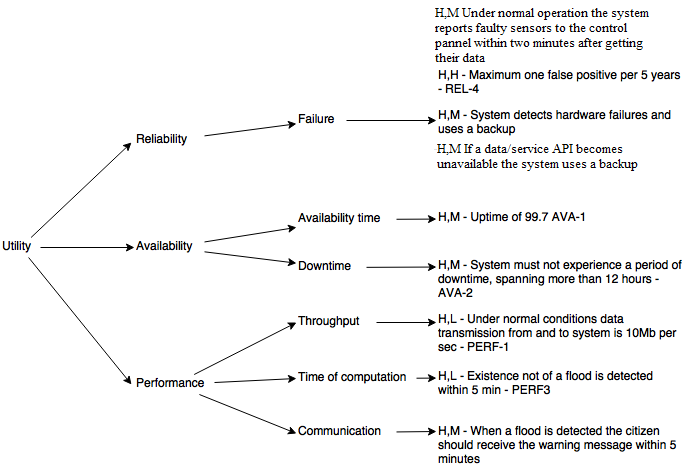
\includegraphics[scale=0.5]{images/utilitytree1.png}

The interesting scenarios are the ones with high priority (H,H),(H,M) and (M,H), focus will be put on them in the next section.
%Using this table we can give points to those scenarios.

\subsection{Scenarios}

In this part high priority scenarios derived from the utility tree will be analysed and as a result will come the identification of sensitivity points, tradeoffs, risks and non risks.


\begin{table}[H]
	\begin{tabular}{L{0.2\textwidth} L{0.6\textwidth}}
		\textbf{Scenario}		& \textbf{Handling faulty sensors} \\ \toprule
		\textbf{Q-Attribute(s)} & Availability, reliability \\ \midrule
		\textbf{Environment} 	& Normal operation \\ \midrule
		\textbf{Stimulus} 		& A sensor sends wrong data or stops sending data \\ \midrule
		\textbf{Response} 		& The system ignores the sensor until is has been repaired/replaced \\ \midrule
		\textbf{Design decisions} 	& \\
			\multicolumn{2}{c}{
			\begin{tabular}{l|lllll}
				\textbf{Decision} & Req. & Sensitiv. & Tradeoff & Risk & Non-Risk \\ \hline
				
				Detection algorithm & \ref{fr:detect-faultysensor}, \ref{rel:2} & \nsl{s}{faultysensor} & \nsl{to}{faultysensor} &  &   \\
				Reporting & \ref{fr:report-faultysensors} &  &  & \nsl{r}{reportfaultysensor} &  \\
				UAV & \ref{fr:uav} & \nsl{s}{uav} & \nsl{to}{uav} & \nsl{r}{uav-weather} & \\
				
			\end{tabular} 
			} \\
			\midrule
			\multicolumn{2}{c}{\compactCell{
				\textbf{Sensitivities:} 
				\begin{itemize} \setlength{\itemsep}{-15pt}
				\item \ref{s:faultysensor}: Some of the time, it will be difficult for the detection algorithm to distinguish between extreme data from a sensor caused by a fault and extreme data caused by a flood.\\
				\item \ref{s:uav}: It takes time for the UAV to be dispatched to the potential flood location.
				\end{itemize} ~\\[-0.5cm]
				\textbf{Tradeoffs:} 
				\begin{itemize} \setlength{\itemsep}{-15pt}
				\item \ref{to:faultysensor}: Reliability (+) vs. Performance (-) -- Using an algorithm on the sensor data to detect faulty sensors adds more overhead, but increases the reliability of the system.\\
				\item \ref{to:uav}: Reliability (+) vs. Performance (-) -- The UAV checks if a flood is present/developing when the sensor data is not conclusive. It has a large dispatch time, which means (if there is a flood), it will be detected with a larger delay. 
				\end{itemize} ~\\[-0.5cm]
				\textbf{Risks:} 
				\begin{itemize} \setlength{\itemsep}{-15pt}
				\item \ref{r:reportfaultysensor}: There is a risk that the config panel where the faulty sensors are reported, is not checked often enough, leading to broken sensors not being replaced.
				\end{itemize}
			}} \\

		\midrule
		\textbf{Reasoning} 		& Temporarily ignoring faulty sensors allows the system to continue functioning. Reporting the sensors using the control panel allows maintenance personnel to repair those sensors. It is important that maintenance personnel checks the control panel regularly. 
		
		In case it cannot be determined by the system if a sensor is faulty, or whether there is a flood, a UAV can be dispatched to check. \\
		%\midrule
		%\textbf{Arch. model} 	&  \\
								 
	 \bottomrule
	\end{tabular}
	\label{ATAM:faulty-sensors}
	\caption{ATAM -- Handling faulty sensors}
\end{table}

\begin{table}[H]
	\begin{tabular}{L{0.2\textwidth} L{0.6\textwidth}}
		\textbf{Scenario}		& \textbf{Handling hardware failures} \\ \toprule
		\textbf{Q-Attribute(s)} & Availability \\ \midrule
		\textbf{Environment} 	& Normal operation \\ \midrule
		\textbf{Stimulus} 		& A hardware component stops operating \\ \midrule
		\textbf{Response} 		& The system uses a backup of the hardware component \\ \midrule
		\textbf{Design decisions} 	& \\
			\multicolumn{2}{c}{
			\begin{tabular}{l|lllll}
				\textbf{Decision} & Req. & Sensitiv. & Tradeoff & Risk & Non-Risk \\ \hline
				
				Database cluster & \ref{ava:1}, \ref{ava:2} &  & \nsl{to}{cluster} &  &   \\
				Analytic cluster & \ref{ava:1}, \ref{ava:2} &  & \ref{to:cluster} &  &  \\
				Multiple data centers & \ref{ava:1}, \ref{ava:2} &  & \nsl{to}{datacentre} &  & \nsl{nr}{datacenters} \\
				Arduino               & \ref{ava:1}, \ref{ava:2} & \nsl{s}{arduinofail} &  &  &  \\
				
			\end{tabular} 
			} \\
			\midrule
			\multicolumn{2}{c}{\compactCell{
				\textbf{Sensitivities:} 
				\begin{itemize} \setlength{\itemsep}{-15pt}
				\item \ref{s:arduinofail}: The Arduino are hardware components which can fail as well. Several sensors are connected to a single Arduino. Since a failing Arduino does not have a backup, those sensors connected to it will become unavailable to the system until the Arduino is repaired. \\
				\end{itemize} ~\\[-1.0cm]
				\textbf{Tradeoffs:} 
				\begin{itemize} \setlength{\itemsep}{-15pt}
				\item \ref{to:cluster}: Availability (+) vs. Affordability (-) -- Using a cluster is more expensive, but provides a fallback in case of failures, increasing the availability. \\
				\item \ref{to:datacentre}: Also Availability (+) vs Affordability (-) -- The costs of the system increase significantly by having a second data center. However, this guarantees the availability of the system in case of problems with one of the data centers.
				\end{itemize} ~\\[-0.5cm]
				\textbf{Nonrisks:} 
				\begin{itemize} \setlength{\itemsep}{-15pt}
				\item \ref{nr:datacenters}: Multiple data centers aid with increasing the availability only when they are not placed in close proximity to each other.
				\end{itemize}
			}} \\

		\midrule
		\textbf{Reasoning} 		& The hardware in the data centers and the data center itself are prepared for failures of components. It is important to note that the data centers should not be placed in close proximity to each other. 
		
		A failure of an Arduino will lead to several sensors going offline, but these sensor are located in a relatively small area and therefore only have a limited impact on the systems monitoring capabilities. \\
		\midrule
		\textbf{Arch. model} 	& See figure~\ref{fig:database-cluster} and figure~\ref{fig:analytic-cluster} for the logical schematic of the database and analytic cluster respectively.
		
		Also see figure~\ref{fig:hardware-archi-schema} for an overview of the multiple data centers. \\
								 
	 \bottomrule
	\end{tabular}
	\caption{ATAM -- Handling hardware failures}
	\label{ATAM:hardware-failure}
\end{table}

\begin{table}[H]
	\begin{tabular}{L{0.2\textwidth} L{0.6\textwidth}}
		\textbf{Scenario}		& \textbf{Ensuring availability of third party data / services} \\ \toprule
		\textbf{Q-Attribute(s)} & Availability, reliability, interoperability \\ \midrule
		\textbf{Environment} 	& Normal operation \\ \midrule
		\textbf{Stimulus} 		& A third party service or data API becomes unavailable \\ \midrule
		\textbf{Response} 		& The system still has access to (a backup of) the data or service \\ \midrule
		\textbf{Design decisions} 	& \\
			\multicolumn{2}{c}{
			\begin{tabular}{l|lllll}
				\textbf{Decision} & Req. & Sensitiv. & Tradeoff & Risk & Non-Risk \\ \hline
				
				Using multiple API providers offering same service/data & \ref{fr:receive-weather}, \ref{fr:receive-geographic} &  & \nsl{to}{apis} &  &   \\
				SMS service & \ref{fr:warn-citizens}, \ref{fr:citizens-subscribe} & \nsl{s}{onesmsservice} &  &  & \nsl{nr}{storingphonenrs}  \\
				Emergency room API & \ref{fr:warn-safetyregion} &  &  &  &  \nsl{nr}{emergencyroomapi} \\
				
				
			\end{tabular} 
			} \\
			\midrule
			\multicolumn{2}{c}{\compactCell{
				\textbf{Sensitivities:} 
				\begin{itemize} \setlength{\itemsep}{-15pt}
				\item \ref{s:onesmsservice}: The system relies on a single SMS Service provider (CM Telecom). If this provider is not available, the system cannot warn citizens by text message. \\
				\end{itemize} ~\\[-1.0cm]
				\textbf{Tradeoffs:} 
				\begin{itemize} \setlength{\itemsep}{-15pt}
				\item \ref{to:apis}: Reliability (+) vs. Affordability (-) -- Most APIs charge a usage fee, which means that using multiple APIs increases the costs. \\
				\end{itemize} ~\\[-1.0cm]
				\textbf{Nonrisks:} 
				\begin{itemize} \setlength{\itemsep}{-15pt}
				\item \ref{nr:storingphonenrs}: The phone numbers of citizens who subscribed are stored in the database of the system instead of the SMS Service provider's database. \\
				\item \ref{nr:emergencyroomapi}: It is assumed that the emergency room API is always available, which is the responsibility of the safety region.
				\end{itemize}
			}} \\

		\midrule
		\textbf{Reasoning} 		& \compactCell{
			By using multiple APIs for weather / geographic / demographic data, it is ensured that this data is available if one of the APIs goes offline. 
			
			The SMS service is a single point of failure: if it goes offline, there is no backup SMS service provider.
		} \\
		%\midrule
		%\textbf{Arch. model} 	& \\
								 
	 \bottomrule
	\end{tabular}
	\caption{ATAM -- Ensuring availability of third party data / services}
	\label{ATAM:3rdpartydata}
\end{table}
